\subsection{MetaDE}

MetaDE package implements 12 major meta-analysis methods with 22 variations for differential expression analysis that fall into 3 main categories: combining p-values, combining effect sizes and others (e.g. combining ranks, etc.). Depending on the type of outcome, the package can perform two class comparison, multi-class comparison, association with continuous or survival outcomes. The package allows the input of either microarray (continuous intensity) and/or RNA-seq data (count) for individual study analysis. 
The R package for MetaDE module can be found at \url{https://github.com/metaOmics/MetaDE}.
After obtaining DE genes from the differential expression analysis, 
users can further perform post-hoc pathway enrichment analysis using the declared DE genes.
In the two subsections below we will go over how to perform (1) differential expression analysis and (2) pathway enrichment analysis based on (1).
Note that 
MetaDE involves many sophisticated meta-analysis methods, please refer to the MetaOmics paper (Supplementary information: Box S3) for a detailed description of each method. 

\subsubsection{Procedure of differential expression analysis}

\begin{figure}[H]
\begin{center}
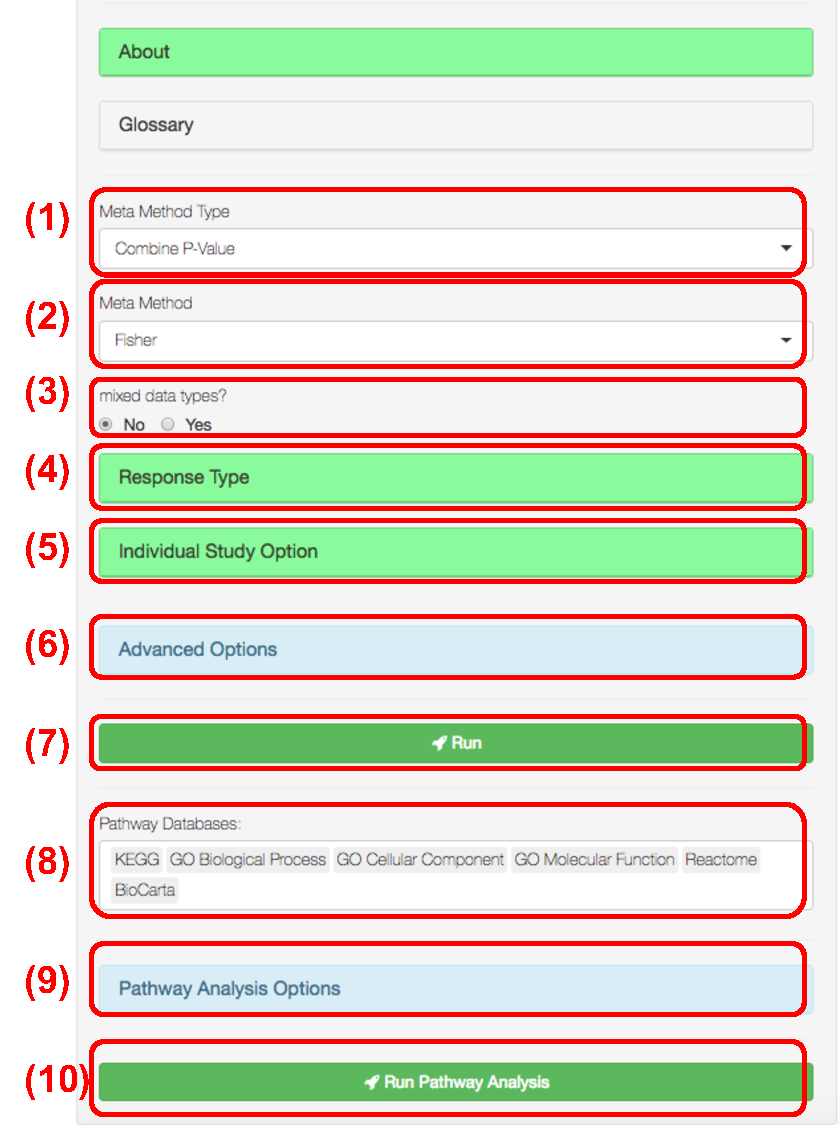
\includegraphics[scale=0.6]{./figure/metaDE/metaDEoption.pdf}
\caption{``MetaDE" options}
\label{fig:MetaDEoption}
\end{center}
\end{figure}

In Figure~\ref{fig:MetaDEoption},
{\color{red} Red boxes (1) - (7)} are the options and steps to run the differential expression analysis.
A detailed list of all options are available in Section~\ref{sec:completeList_MetaDE}. 

\begin{steps}
\item \textbf{Choose the type of meta-analysis method:}
There are three types of meta-analysis to choose:
combining p-values, combining effect size and others.

\item \textbf{Choose a meta-analysis method:}
\begin{itemize}
\item For ``combining p-values" category,
users can choose from ``Fisher", ``AW-Fisher$^{\ast}$", ``maxP", ``minP", ``rOP$^{\ast}$" and ``Stouffer",
where some of them have the one-sided corrected versions. 

\item For ``combining effect size" category,
users can choose from ``FEM" and ``REM$^{\ast}$",
where ``REM$^{\ast}$" has choice of six analytical algorithms for implementation.

\item For ``others",
there are three rank-based method (PR, SR and rankProd) and minMCC for multi-class meta-analysis.
To choose from the overwhelmingly many meta-analysis methods,
we follow \cite{chang2013meta} and mark * for top performing methods AW-Fisher, REM (HO option) and rOP as recommendation for users.
\end{itemize}

\item \textbf{Mixed data type:}
If this option is selected,
MetaDE will allow partial studies with count data from RNA-seq and remaining studies with continuous intensities from microarray.

\item \textbf{Choose the response type:}
Under the drop-down menu,
users can specify types of outcome (response) variable to be two-class, continuous, multi-class or survival.
By choosing ``two class comparison",
users can specify the group label name for the Label Attribute (from the column names of your clinical data).
Then for group label (a factor of at least two levels),
specify the name for the ``Control Label" and ``Experimental Label", respectively.
For the other types, only group label name is needed.

\item \textbf{Choose Study Design for individual study:}
\begin{itemize}
\item Individual data type can be either discrete (count) or continuous.
\item Under drop-down menu ``Setting Individual Study method", user can specify  individual study method according to individual data type.
For continuous data (e.g. microarray), available options include LIMMA (default method) and SAM.
For discrete data (e.g. RNA-seq count), available options include edgeR, DESeq2 and voom.
\item The users can also specify whether each study is paired design or not.
\end{itemize}

\item \textbf{Advanced Options}
\begin{itemize}
\item Use complete options: other uncommonly used options will become available. Again, this is not suggested if you are not familiar with the method.
\item Parametric: if No is selected, permutation will be performed instead of parametric closed form solution.
\item Covariate: indicate if any covariate will be adjusted.
\item Alternative Hypothesis: two-sided or one-sided.
\end{itemize}

\item \textbf{Run:}
Once all the above options are specified, users can click on ``Run" button to perform MetaDE analysis

\end{steps}

\subsubsection{Results of differential expression analysis}

We used the AML example to demonstrate the MetaDE module.
After merging the three datasets and filtering out 50\% of genes by mean and 50\% of genes by variance, 1283 genes remained.
In this example we only compared two phenotypes: inv(16) and t(15;17).
Detailed descriptions of these studies can be found in Table~\ref{tab:realDataLeukemia}. 
Two main outputs from the first ``meta differential analysis" step in the procedure are shown in Figure \ref{fig:MetaDEresult1}. 


\begin{figure}[H]
\begin{center}
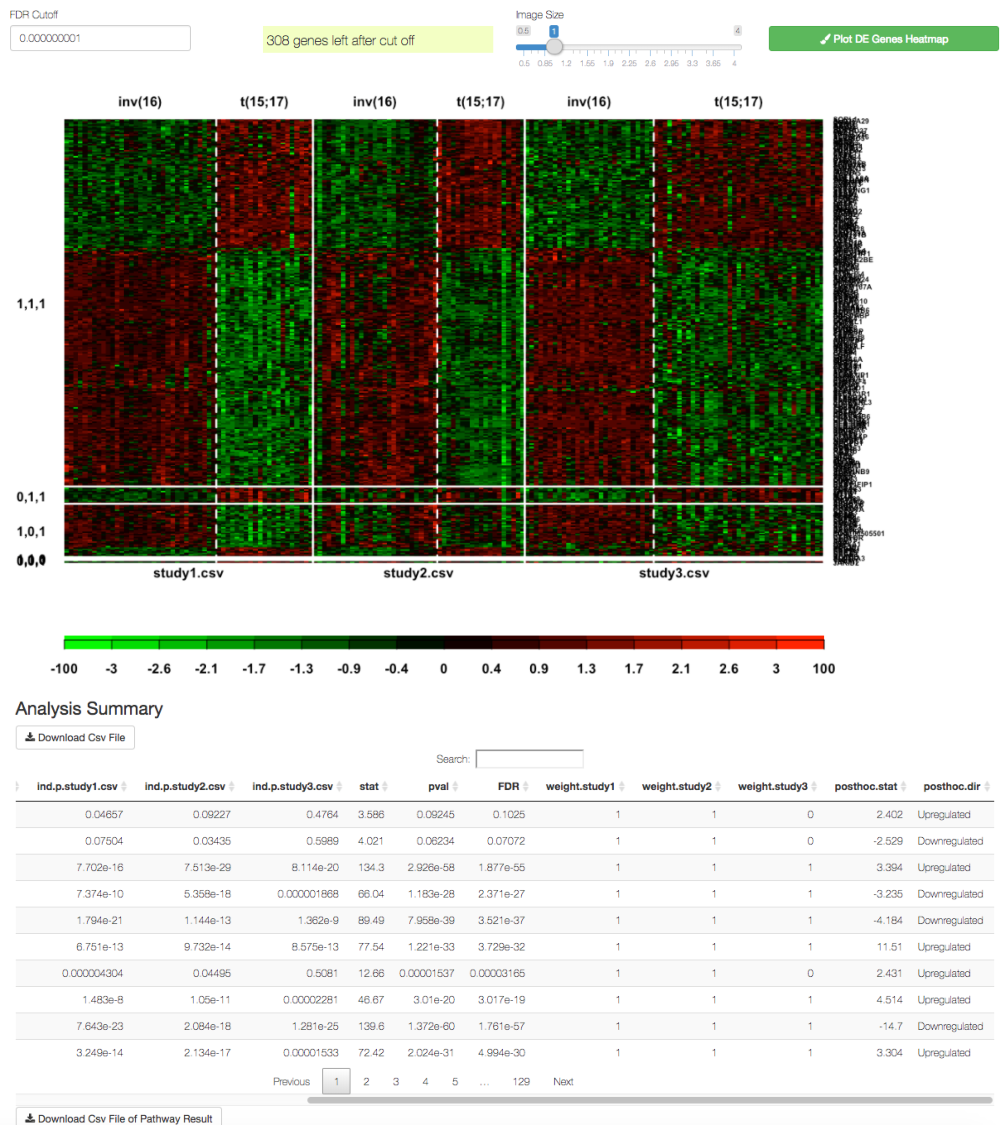
\includegraphics[scale=1]{./figure/metaDE/metaDEresult.pdf}
\caption{``MetaDE" Results.
Heatmap of DE genes is rendered after specifying the FDR cutoff for selection of DE genes and clicking on ``Plot DE Genes Heatmap". 
The ``image size" can be adjusted by dragging the scroll bar. 
In the heatmap, rows refer to the declared DE genes under the specified FDR cutoff, 
columns refer to samples, and solid white lines are used to separate different studies and the dashed white lines are used to separate groups. 
Colors of the cells correspond to scaled expression level as indicated in the color key below. 
For the results generated by ``AW-Fisher$^{\ast}$", there is one additional column of cross-study weight distribution on the left end of the heatmap and the genes in the heatmap are sorted by their weight distribution.
Summary of meta analysis results is on bottom, 
including information of individual test statistics, individual study p-value, meta-analysis p-value, FDR, etc. 
}
\label{fig:MetaDEresult1}
\end{center}
\end{figure}

\subsubsection{Procedure of downstream pathway analysis}
Users can then perform pathway enrichment analysis on the declared DE genes from the previous step, 
the options and steps of which are shown in {\color{red} Red boxes (8) - (10)} in Figure~\ref{fig:MetaDEoption}.
Procedure is outlined as below.

\begin{steps}
\item \textbf{Choose the pathway database:}
Users can select from 25 available pathway databases to perform the pathway enrichment analysis. 

\item \textbf{Choose the pathway enrichment method and the pathway size range:}
In this step users can choose pathway enrichment options with Kolmogorov-Smirnov (KS) test as default option,
or Fisher's exact test by specifying number of input genes for pathway analysis.
Both of these two tests could provide significance measurement on DE gene enrichment in the pre-specified pathways.
For Fisher's exact test, the input genes can be obtained by either specifying a MetaDE p-value cutoff, or specifying number of top DE genes.
KS-test doesn't require a specific p-value cutoff as it will use all MetaDE p-value information to test the enrichment.
Users can also specify the minimum/maximum gene size of pathways to be included for pathway enrichment analysis.

\item \textbf{Run:}
Once all the above options are specified, users can click on ``Run Pathway analysis" button to perform pathway enrichment analysis.

\end{steps}


\subsubsection{Result of downstream pathway analysis}

The result for downstream pathway analysis is shown in Figure \ref{fig:MetaDEresult2}. 
The summary includes the pathway names, the corresponding enrichment p-value and FDR. 
In addition to the results shown in the browser, 
users can download the result by clicking on "Download Csv File" on the top left of the summary table. 

\begin{figure}[H]
\begin{center}
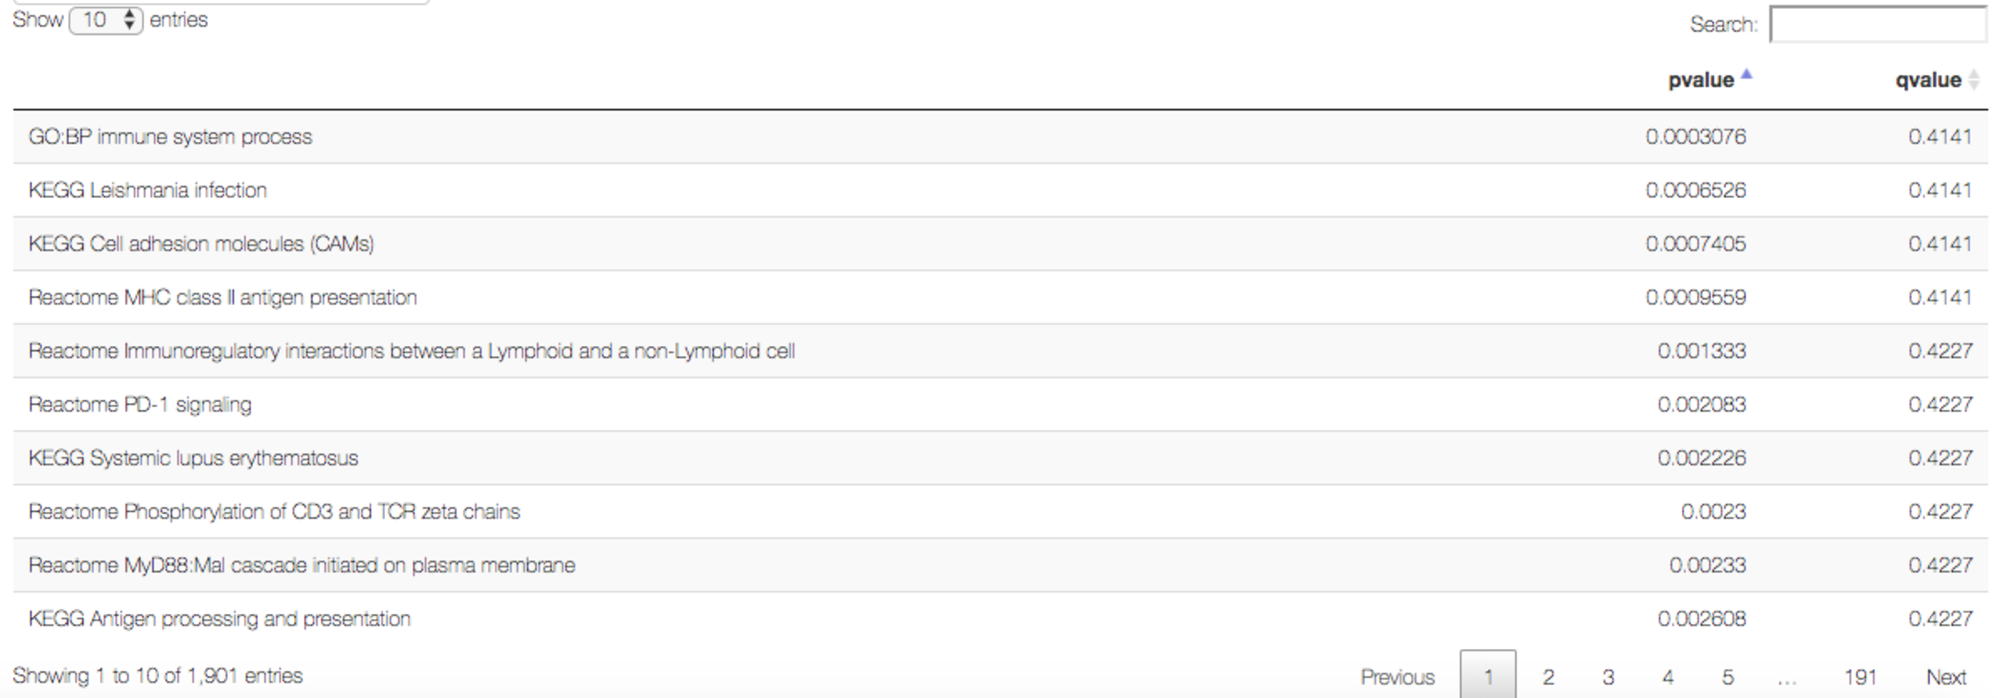
\includegraphics[scale=0.5]{./figure/metaDE/MetaDE_pathway.pdf}
\caption{Downstream pathway analysis based on MetaDE genes.
Each row represents a pathway with its p-value and q-value listed on the right.
}
\label{fig:MetaDEresult2}
\end{center}
\end{figure}



